\documentclass{article}
\usepackage{iclr2027_conference,times}
\input{math_commands.tex}
\usepackage{amsmath,amssymb,amsthm,booktabs,multirow,graphicx,xcolor}
\usepackage{tikz}
\usetikzlibrary{arrows.meta,calc,fit,positioning,shapes.geometric}
\usepackage{microtype}
\usepackage{hyperref}
\usepackage{url}

\newcommand{\method}{\textsc{GAR-JEPA}}
\newcommand{\gar}{\textsc{GAR}}
\newcommand{\todoresult}{\textcolor{gray}{\textit{pending}}}
\newcommand{\privileged}{\textsuperscript{\dag}}
\newtheorem{proposition}{Proposition}
\newtheorem{corollary}{Corollary}

\title{Prediction Is Not Planning:\\Geometric Advantage Ranking for Language-Action JEPAs}

\author{Anonymous authors}

% Keep anonymous for submission.
% \iclrfinalcopy

\begin{document}
\maketitle

\begin{abstract}
Agents that act through language must compare consequences, not only generate plausible text. We study action-conditioned joint-embedding prediction in a controlled language-mediated planning environment. We first formalize a planning state as an equivalence class of histories with identical controlled futures. This predictive state is sufficient for control, but its geometry is not identified by transition prediction. Equally predictive re-embeddings can reverse which successor appears closest to a goal. We introduce Geometric Advantage Ranking (GAR), a training objective that imposes within-state order constraints on counterfactual action consequences. GAR can supervise a scorer that factors through a predicted successor or a matched direct scorer. On stylized arithmetic dependency puzzles, a non-generative JEPA solves $43.3\%$ of episodes in the minimum number of actions under a common feasible-action interface. The strongest sentence model reaches $52.1\%$, so our result establishes viability rather than superiority. The central finding concerns mechanism. Latent prediction alone reaches $18.3\%$, while the complete predictive GAR model reaches $43.3\%$. Five-seed ablations show that counterfactual ordering and successor prediction contribute complementary information. Local action-order diagnostics are more favorable for the learned GAR score than for raw latent distance, while global effective rank does not explain planning. These results support a narrow conclusion: prediction can supply a useful state, but planning requires additional structure that orders action consequences.
\end{abstract}

\section{Introduction}

Language agents are commonly trained to predict which words come next, even when their task is to choose an action according to its consequences. We ask whether an agent can instead predict the latent consequence of each language action and plan with those predicted states. This question separates two capabilities that autoregressive generation usually entangles. A model must represent what has happened, and it must order the actions that remain.

Joint-embedding predictive architectures provide a natural substrate for the first capability \citep{lecun2022path,assran2023ijepa}. An action-conditioned predictor maps the current representation and a language action to a predicted successor representation. Such a model can preserve consequence-relevant information without reconstructing every word. Action-conditioned JEPAs have already supported planning in physical environments \citep{assran2025vjepa2}. Language actions raise a focused question. If the next latent state is predicted accurately, does its geometry support choosing an action?

The answer is not automatic. Predictive learning can identify which histories have the same controlled future, but it need not identify a metric that ranks different futures by progress toward a goal. A bijective re-embedding preserves every latent transition and can still reverse the distances of two successor states to the goal. Prediction gives a state representation. It does not by itself give a planning geometry.

We study this gap in a controlled language-action testbed. Each stylized iGSM episode presents an arithmetic dependency problem. At each step, every learned method receives the same shuffled menu of executable intent phrases. The environment executes the selected phrase and returns its textual consequence. Supplying the current feasible menu is an intentional laboratory intervention. It holds proposal and syntactic validity fixed so that the experiment compares how learning objectives value the same language actions.

We introduce Geometric Advantage Ranking (GAR). GAR uses factual and counterfactual action outcomes to impose local order constraints among candidate consequences. In the main JEPA, a scorer consumes the predicted successor. In a matched direct GAR control, the scorer consumes the history and action without using the predicted successor in its policy path. This terminology separates the supervision from the architectural factorization.

Our empirical goal is explanatory rather than competitive. A predictive GAR JEPA attains $43.3\%$ strict success over five seeds. A token language model attains $42.2\%$, a sentence language model attains $47.1\%$, and a sentence model with an auxiliary latent objective attains $52.1\%$. The JEPA is therefore a viable planner under the shared interface, but it is not the best model. The more informative result is that latent prediction alone attains $18.3\%$. The full method attains $43.3\%$, and removing the GAR terms attains $7.6\%$. Counterfactual ordering is the main source of the gain, while counterfactual successor prediction provides an additional benefit.

The paper develops one connected argument.
\begin{enumerate}
    \item We define the state needed for language-mediated control as a quotient of histories that have identical controlled futures, and show why this state is control sufficient.
    \item We show that exact latent transition prediction does not identify a goal-directed metric without further assumptions. GAR supplies local counterfactual order constraints that are sufficient for strict planning when they recover the optimal action ordering.
    \item We test the mechanism with five-seed objective ablations, gradient-routing controls, matched GAR scorers, and representation diagnostics. The evidence supports GAR as useful ordering supervision. It does not yet establish that successor factorization is uniformly better than direct scoring.
\end{enumerate}

The resulting claim is deliberately narrow: action-conditioned latent prediction can support language-action planning, but predictive accuracy alone leaves the decision geometry underdetermined.

\section{Predictive States and Planning Geometry}
\label{sec:framework}
\label{sec:method}

\paragraph{Language-mediated control.}
Language provides many surface forms for the same situation. ``The number of red objects is six'' and ``There are six red objects'' may support exactly the same future calculations. Replacing either sentence by ``There are not six red objects'' can change every valid continuation. A useful state representation should ignore the first wording change and preserve the second semantic change.

We model this setting as a controlled process
\begin{equation}
    \mathcal{M}=(\mathcal{S},\mathcal{U},P,\Omega,O,c,\mathcal{G}).
\end{equation}
The semantic state is $s_t\in\mathcal{S}$ and a semantic intervention is $u_t\in\mathcal{U}$. The agent receives a language observation $x_t\in\Omega$ and chooses a language action $a_t$. A grounding map $\alpha(a_t)=u_t$ connects the phrase to its effect. Decisions may depend on the full history
\begin{equation}
    h_t=(x_0,a_0,x_1,\ldots,a_{t-1},x_t),
\end{equation}
rather than on the latest sentence alone. Histories accommodate synonymous descriptions, irrelevant facts, and partial observations without requiring a network to recover a privileged hidden coordinate system.

\paragraph{Predictive equivalence.}
Predictive state representations define state through action-conditioned predictions of future observations \citep{littman2001predictive}. Let $Y$ collect future task-relevant observations and terminal outcomes, let $C$ collect future costs, and let $F$ collect future feasible-action sets. Histories $h$ and $h'$ are controlled-predictively equivalent when every policy over actions admissible from both histories induces the same future law:
\begin{align}
h \sim_{\mathrm{pred}} h'
\quad\Longleftrightarrow\quad
\mathcal{L}_{\pi}(Y_{t+1:\tau},C_{t:\tau},F_{t:\tau}\mid h)
=
\mathcal{L}_{\pi}(Y_{t+1:\tau},C_{t:\tau},F_{t:\tau}\mid h')
\quad\forall\pi.
\label{eq:predictive-equivalence}
\end{align}
The corresponding predictive state is the equivalence class
\begin{equation}
    q(h)=[h]_{\sim_{\mathrm{pred}}}\in\mathcal{H}/{\sim_{\mathrm{pred}}}.
\end{equation}
Histories with identical controlled futures meet in the quotient even when their wording differs. A negation, operator substitution, or changed entity relation remains visible whenever it changes a future consequence. Information that cannot affect any future task outcome may disappear.

\begin{proposition}[Control sufficiency]
If $h\sim_{\mathrm{pred}}h'$ includes equality of future costs and terminal events under every admissible policy, then $V^\pi(h)=V^\pi(h')$ for every policy $\pi$, and therefore $V^\star(h)=V^\star(h')$.
\end{proposition}
\begin{proof}
Return is a function of the future cost and terminal sequence. Equation~\ref{eq:predictive-equivalence} assigns that sequence the same distribution under each policy. Its expectation is therefore equal. Maximizing over policies preserves the equality.
\end{proof}

Proposition 1 defines the state required for control. We do not claim it as a new control theorem. Bisimulation gives a related recursive characterization through agreement in immediate reward and transitions between equivalence classes \citep{ferns2011bisimulation}. GAR imposes a narrower condition, namely goal-conditioned order among actions available at one history.

The experiments instantiate the framework with a deterministic finite-horizon process. Executing $a$ appends one deterministic textual consequence, written $T(h,a)$. Stochastic environments would require a predictive distribution or another representation of multimodal futures. A point predictor trained by mean-squared error generally represents only a conditional mean.

\paragraph{Coordinate ambiguity.}
Suppose an encoder $\phi$ and predictor $F$ recover every deterministic transition:
\begin{equation}
    F(\phi(h),e(a))=\phi(T(h,a)).
\end{equation}

\begin{proposition}[Predictive ambiguity]
Let $b$ be a bijection on the realized latent states and define $\widetilde\phi=b\circ\phi$ together with
\begin{equation}
    \widetilde F(b(z),e(a))=b(F(z,e(a))).
\end{equation}
Then $(\widetilde\phi,\widetilde F)$ predicts the same realized transitions exactly. A non-isometric $b$ need not preserve the order of successor distances to a goal.
\end{proposition}
\begin{proof}
Substitution gives $\widetilde F(\widetilde\phi(h),e(a))=\widetilde\phi(T(h,a))$. On a finite realized state set, the images of two successors and a goal may be placed at arbitrary distinct points. Their goal-distance order can change without changing any transition identity.
\end{proof}

The two embeddings in Figure~\ref{fig:nonidentifiability} realize the same transitions and disagree on the preferred successor. Additional assumptions can reduce this ambiguity. For example, controlled Gaussian world models with spectral separation and sufficient conditional action excitation can be identified up to an orthogonal map \citep{song2026identifiability}. Proposition 2 concerns predictive learning without such metric-preserving guarantees.

\paragraph{Predictive architecture.}
The online encoder produces $z_h=\phi_\theta(h)$ and the action encoder produces $e_\theta(a)$. Their predicted successor is
\begin{equation}
    \widehat z_{h,a}=F_\theta(z_h,e_\theta(a)).
\end{equation}
An exponential-moving-average encoder maps each observed successor history to a stopped-gradient target $\bar z_{T(h,a)}$. Factual and counterfactual prediction losses match $\widehat z_{h,a}$ to these targets. The target encoder stays in evaluation mode and every dropout rate is zero.

At inference time, the prompt and query are represented by a problem anchor $z_x$. The transition-value realization assigns a lower-is-better energy
\begin{equation}
    E^{\mathrm{TV}}_\psi(h,a,x)=V_\psi(\widehat z_{h,a},z_x).
\end{equation}
The policy predicts and scores every currently feasible phrase, then selects the minimum-energy candidate. Figure~\ref{fig:method} separates this inference path from the training signals.

\begin{figure}[t]
    \centering
    \resizebox{0.96\linewidth}{!}{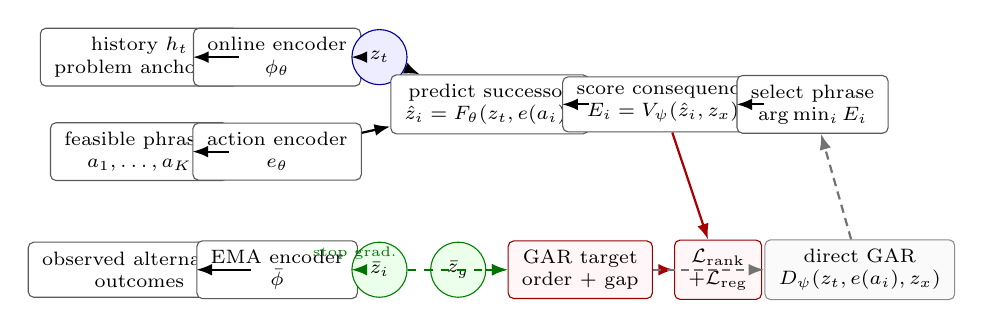
\begin{tikzpicture}[
    x=1cm,y=1cm,
    box/.style={draw=black!65,rounded corners=2pt,fill=white,minimum height=7mm,align=center,font=\scriptsize,inner xsep=5pt},
    latent/.style={circle,draw=blue!60!black,fill=blue!7,minimum size=7mm,font=\scriptsize},
    target/.style={circle,draw=green!50!black,fill=green!8,minimum size=7mm,font=\scriptsize},
    arrow/.style={-{Latex[length=2mm]},thick},
    targetarrow/.style={-{Latex[length=2mm]},thick,green!45!black,dashed},
    control/.style={-{Latex[length=2mm]},thick,black!55,densely dashed}
]
% Deployed predictive policy path
\node[box] (history) at (0,2.15) {history $h_t$\\problem anchor $x$};
\node[box] (encoder) at (1.75,2.15) {online encoder\\$\phi_\theta$};
\node[latent] (state) at (3.05,2.15) {$z_t$};
\node[box] (actions) at (0,0.95) {feasible phrases\\$a_1,\ldots,a_K$};
\node[box] (aenc) at (1.75,0.95) {action encoder\\$e_\theta$};
\node[box] (pred) at (4.45,1.55) {predict successor\\$\hat z_i=F_\theta(z_t,e(a_i))$};
\node[box] (value) at (6.65,1.55) {score consequence\\$E_i=V_\psi(\hat z_i,z_x)$};
\node[box] (choice) at (8.55,1.55) {select phrase\\$\arg\min_i E_i$};
\draw[arrow] (history) -- (encoder);
\draw[arrow] (encoder) -- (state);
\draw[arrow] (state) -- (pred);
\draw[arrow] (actions) -- (aenc);
\draw[arrow] (aenc) -- (pred);
\draw[arrow] (pred) -- (value);
\draw[arrow] (value) -- (choice);

% Training target path
\node[box] (outcomes) at (0,-0.55) {observed alternative\\outcomes};
\node[box] (ema) at (1.75,-0.55) {EMA encoder\\$\bar\phi$};
\node[target] (next) at (3.05,-0.55) {$\bar z_i$};
\node[target] (goal) at (4.05,-0.55) {$\bar z_g$};
\node[box,draw=red!60!black,fill=red!3] (gar) at (5.6,-0.55) {GAR target\\order + gap};
\node[box,draw=red!60!black,fill=red!3] (loss) at (7.35,-0.55) {$\mathcal L_{\rm rank}$\\$+\mathcal L_{\rm reg}$};
\draw[arrow] (outcomes) -- (ema);
\draw[targetarrow] (ema) -- node[above,font=\tiny] {stop grad.} (next);
\draw[targetarrow] (next) -- (gar);
\draw[targetarrow] (goal) -- (gar);
\draw[arrow,red!65!black] (gar) -- (loss);
\draw[arrow,red!65!black] (value) -- (loss);

% Information-matched architectural control
\node[box,draw=black!45,fill=black!2] (direct) at (9.15,-0.55) {direct GAR\\$D_\psi(z_t,e(a_i),z_x)$};
\draw[control] (gar) -- (direct);
\draw[control] (direct) -- (choice);
\end{tikzpicture}
}
    \caption{Inference and training paths for predictive GAR. At inference, each candidate phrase is encoded, passed through the successor predictor, and scored against the problem anchor. Training observes factual and counterfactual successor histories. EMA target distances define within-state order labels, while latent prediction preserves the action-conditioned transition.}
    \label{fig:method}
\end{figure}

\paragraph{Geometric Advantage Ranking.}
Let $\bar z_g$ be the EMA representation of the terminal training history. Each observed candidate successor receives the target distance
\begin{equation}
    \bar d_i=d(\bar z_{T(h,a_i)},\bar z_g).
\end{equation}
The default target evaluates a candidate after a bounded two-step reference continuation. It remains a geometric progress surrogate rather than a Bellman-consistent advantage. Whether its order agrees with true continuation quality is measured directly in the action audits.

Whenever $\bar d_i+\epsilon<\bar d_j$, GAR imposes
\begin{equation}
    \mathcal{L}_{\mathrm{rank}}
    =\sum_{i\succ j}\left[m+E_\psi(h,a_i,x)-E_\psi(h,a_j,x)\right]_+.
\end{equation}
A calibration term matches differences in predicted energy to differences in target distance:
\begin{equation}
    \mathcal{L}_{\mathrm{reg}}
    =\sum_{i<j}\left[(E_j-E_i)-\beta(\bar d_j-\bar d_i)\right]^2.
\end{equation}
Together with factual and counterfactual latent prediction, the training objective is
\begin{equation}
    \mathcal{L}=\mathcal{L}_{\mathrm{factual}}
    +\lambda_{\mathrm{cf}}\mathcal{L}_{\mathrm{cf}}
    +\lambda_{\mathrm{rank}}\mathcal{L}_{\mathrm{rank}}
    +\lambda_{\mathrm{reg}}\mathcal{L}_{\mathrm{reg}}.
\end{equation}
GAR gradients reach the scorer, predictor, action encoder, and online history encoder in the default model. The EMA network follows the online encoder without receiving gradients.

GAR names the supervision, not the scorer architecture. Transition-value GAR factors the energy through $\widehat z_{h,a}$. Direct GAR uses $D_\psi(z_h,e(a),z_x)$ and bypasses the successor in the policy path. Raw-distance GAR uses $d(\widehat z_{h,a},\bar z_g)$ without a learned head. The last variant receives the terminal training representation during evaluation and is reported only as an oracle-terminal diagnostic.

\paragraph{Local planning condition.}
Let $D^\star(h)$ denote the shortest remaining action count in a deterministic unit-cost puzzle, and define
\begin{equation}
    A^\star(h,a)=D^\star(h)-1-D^\star(T(h,a)).
\end{equation}
An action on a shortest solution has $A^\star=0$. An action that spends a step without reducing the remaining distance has $A^\star=-1$.

\begin{proposition}[Local ordering]
If a learned score ranks every optimal action above every suboptimal action at every reachable history, greedy selection reaches the goal in exactly $D^\star(h_0)$ actions.
\end{proposition}
\begin{proof}
At remaining distance $d>0$, the selected action reaches a history with distance $d-1$. Repeating the argument reaches distance zero after $d$ actions.
\end{proof}

If the smallest true action gap is $\gamma>0$, a uniform estimation error below $\gamma/2$ preserves the same ordering. GAR does not receive $A^\star$ during main training. The proposition instead identifies the behavioral condition that its geometric labels must recover. Pairwise ordering, top-1 recall, regret, and margin therefore provide more direct tests than effective rank or global probe accuracy.

\paragraph{Compression.}
The quotient is the coarsest exact partition that preserves controlled futures. It supplies a formal notion of task-relevant compression, but the neural encoder is not guaranteed to find that minimum. The information bottleneck likewise seeks a compressed code that preserves target information \citep{tishby2000information}. Our objective contains no rate penalty, so latent width and effective rank cannot be interpreted as evidence for an explicit information bottleneck.

\section{From predictive state to planning geometry}
\label{sec:method}

\subsection{Prediction leaves the metric underdetermined}

Let an encoder $\phi$ map a history to $z_h$, let $e(a)$ encode a language action, and let $F$ predict the deterministic successor:
\begin{equation}
    F(\phi(h),e(a))=\phi(T(h,a)).
\end{equation}

\begin{proposition}[Exact prediction does not identify planning geometry]
Suppose $(\phi,F)$ predicts every realized transition exactly. Let $b$ be any bijection on the realized latent states. Define $\widetilde\phi=b\circ\phi$ and
\begin{equation}
    \widetilde F(b(z),e(a))=b(F(z,e(a))).
\end{equation}
Then $(\widetilde\phi,\widetilde F)$ is also prediction perfect. Unless $b$ preserves the chosen metric, it need not preserve the order of successor distances to a goal. On a finite realized state set, a bijection can reverse the goal-distance ordering of two successors while retaining every transition.
\end{proposition}
\begin{proof}
Substitution gives $\widetilde F(\widetilde\phi(h),e(a))=b(\phi(T(h,a)))=\widetilde\phi(T(h,a))$. For two distinct successor states and a goal, assign their images to any three distinct points. Choosing the first successor farther from the goal than the second reverses their metric order without changing the transition identity.
\end{proof}

Figure~\ref{fig:nonidentifiability} shows the consequence. This proposition applies without extra identifiability assumptions or planning-aware constraints. Controlled world models can be identifiable up to more restricted maps, including orthogonal transformations, under strong structural and excitation assumptions \citep{song2026identifiability}.

\begin{figure}[t]
    \centering
    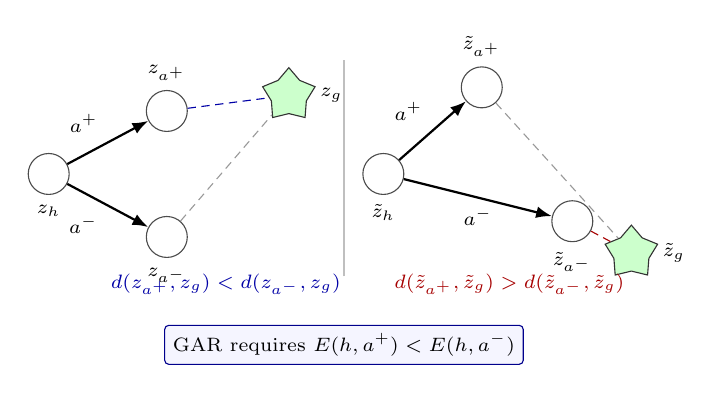
\begin{tikzpicture}[
    x=1cm,y=1cm,
    state/.style={circle,draw=black!70,fill=white,minimum size=5.2mm,inner sep=0pt},
    goal/.style={star,star points=5,draw=black!80,fill=green!20,minimum size=7mm,inner sep=0pt},
    action/.style={-{Latex[length=2mm]},thick},
    preference/.style={-{Latex[length=2mm]},very thick,blue!65!black},
    note/.style={font=\scriptsize,align=center}
]
\node[state,label=below:{\scriptsize $z_h$}] (h1) at (0.5,1.45) {};
\node[state,label=above:{\scriptsize $z_{a^+}$}] (p1) at (2.0,2.25) {};
\node[state,label=below:{\scriptsize $z_{a^-}$}] (n1) at (2.0,0.65) {};
\node[goal,label=right:{\scriptsize $z_g$}] (g1) at (3.55,2.45) {};
\draw[action] (h1) -- node[above left,font=\scriptsize] {$a^+$} (p1);
\draw[action] (h1) -- node[below left,font=\scriptsize] {$a^-$} (n1);
\draw[blue!65!black,densely dashed] (p1) -- (g1);
\draw[black!40,densely dashed] (n1) -- (g1);

\draw[black!25,thick] (4.25,0.15) -- (4.25,2.9);

\node[state,label=below:{\scriptsize $\tilde z_h$}] (h2) at (4.75,1.45) {};
\node[state,label=above:{\scriptsize $\tilde z_{a^+}$}] (p2) at (6.0,2.55) {};
\node[state,label=below:{\scriptsize $\tilde z_{a^-}$}] (n2) at (7.15,0.85) {};
\node[goal,label=right:{\scriptsize $\tilde z_g$}] (g2) at (7.9,0.45) {};
\draw[action] (h2) -- node[above left,font=\scriptsize] {$a^+$} (p2);
\draw[action] (h2) -- node[below,font=\scriptsize] {$a^-$} (n2);
\draw[black!40,densely dashed] (p2) -- (g2);
\draw[red!65!black,densely dashed] (n2) -- (g2);

\node[note,blue!65!black] at (2.75,0.05) {$d(z_{a^+},z_g)<d(z_{a^-},z_g)$};
\node[note,red!65!black] at (6.35,0.05) {$d(\tilde z_{a^+},\tilde z_g)>d(\tilde z_{a^-},\tilde z_g)$};
\node[note,draw=blue!55!black,rounded corners=1.5pt,fill=blue!4,inner sep=3pt] at (4.25,-0.72)
{GAR requires $E(h,a^+)<E(h,a^-)$};
\end{tikzpicture}

    \caption{Transition prediction fixes which successor follows each action, but not how successors are arranged relative to the goal. Both embeddings have zero transition error. GAR adds an order constraint that excludes the right-hand arrangement for the illustrated preference.}
    \label{fig:nonidentifiability}
\end{figure}

\subsection{Action-conditioned joint-embedding prediction}

The online encoder produces $z_h=\phi_\theta(h)$ and the action encoder produces $e_\theta(a)$. The predictor gives
\begin{equation}
    \widehat z_{h,a}=F_\theta(z_h,e_\theta(a)).
\end{equation}
An exponential-moving-average encoder produces a stopped-gradient target $\bar z_{T(h,a)}$. The factual and counterfactual prediction terms minimize normalized latent error for observed successor histories. The target encoder is always in evaluation mode and all dropout is disabled.

\begin{figure}[t]
    \centering
    \resizebox{\linewidth}{!}{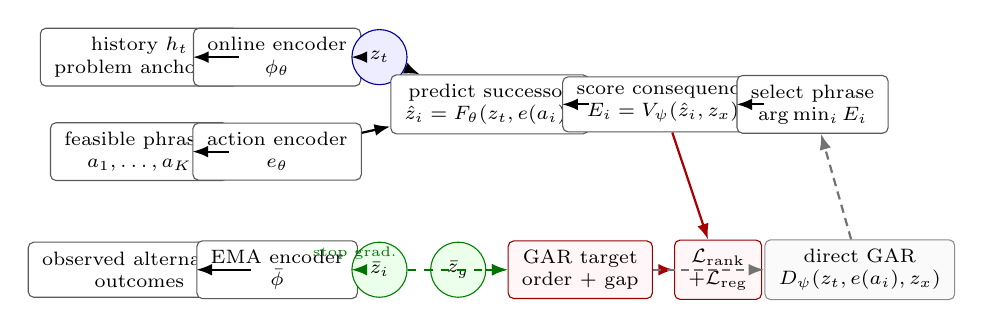
\begin{tikzpicture}[
    x=1cm,y=1cm,
    box/.style={draw=black!65,rounded corners=2pt,fill=white,minimum height=7mm,align=center,font=\scriptsize,inner xsep=5pt},
    latent/.style={circle,draw=blue!60!black,fill=blue!7,minimum size=7mm,font=\scriptsize},
    target/.style={circle,draw=green!50!black,fill=green!8,minimum size=7mm,font=\scriptsize},
    arrow/.style={-{Latex[length=2mm]},thick},
    targetarrow/.style={-{Latex[length=2mm]},thick,green!45!black,dashed},
    control/.style={-{Latex[length=2mm]},thick,black!55,densely dashed}
]
% Deployed predictive policy path
\node[box] (history) at (0,2.15) {history $h_t$\\problem anchor $x$};
\node[box] (encoder) at (1.75,2.15) {online encoder\\$\phi_\theta$};
\node[latent] (state) at (3.05,2.15) {$z_t$};
\node[box] (actions) at (0,0.95) {feasible phrases\\$a_1,\ldots,a_K$};
\node[box] (aenc) at (1.75,0.95) {action encoder\\$e_\theta$};
\node[box] (pred) at (4.45,1.55) {predict successor\\$\hat z_i=F_\theta(z_t,e(a_i))$};
\node[box] (value) at (6.65,1.55) {score consequence\\$E_i=V_\psi(\hat z_i,z_x)$};
\node[box] (choice) at (8.55,1.55) {select phrase\\$\arg\min_i E_i$};
\draw[arrow] (history) -- (encoder);
\draw[arrow] (encoder) -- (state);
\draw[arrow] (state) -- (pred);
\draw[arrow] (actions) -- (aenc);
\draw[arrow] (aenc) -- (pred);
\draw[arrow] (pred) -- (value);
\draw[arrow] (value) -- (choice);

% Training target path
\node[box] (outcomes) at (0,-0.55) {observed alternative\\outcomes};
\node[box] (ema) at (1.75,-0.55) {EMA encoder\\$\bar\phi$};
\node[target] (next) at (3.05,-0.55) {$\bar z_i$};
\node[target] (goal) at (4.05,-0.55) {$\bar z_g$};
\node[box,draw=red!60!black,fill=red!3] (gar) at (5.6,-0.55) {GAR target\\order + gap};
\node[box,draw=red!60!black,fill=red!3] (loss) at (7.35,-0.55) {$\mathcal L_{\rm rank}$\\$+\mathcal L_{\rm reg}$};
\draw[arrow] (outcomes) -- (ema);
\draw[targetarrow] (ema) -- node[above,font=\tiny] {stop grad.} (next);
\draw[targetarrow] (next) -- (gar);
\draw[targetarrow] (goal) -- (gar);
\draw[arrow,red!65!black] (gar) -- (loss);
\draw[arrow,red!65!black] (value) -- (loss);

% Information-matched architectural control
\node[box,draw=black!45,fill=black!2] (direct) at (9.15,-0.55) {direct GAR\\$D_\psi(z_t,e(a_i),z_x)$};
\draw[control] (gar) -- (direct);
\draw[control] (direct) -- (choice);
\end{tikzpicture}
}
    \caption{The predictive GAR factorization. The model encodes a language history, predicts one successor for each feasible phrase, and applies same-state GAR supervision. The transition-value realization scores predicted successors. A matched direct GAR realization bypasses the successor only in the policy path.}
    \label{fig:method}
\end{figure}

\subsection{Geometric Advantage Ranking}

Let $z_g$ denote a target representation and define a latent potential $\Phi_g(z)=-d(z,z_g)$. The geometric progress of an action is
\begin{equation}
    \Delta_\theta(h,a;g)=d(z_h,z_g)-d(\widehat z_{h,a},z_g).
\end{equation}
For candidates $a_i$ and $a_j$, GAR uses observed counterfactual outcomes to derive a stopped-gradient preference label. In the implemented geometric target, each true successor is encoded by the EMA network and compared with the episode's terminal EMA state. The default horizon-two target extends this comparison with a bounded reference continuation. It is a geometric progress surrogate, not a Bellman-consistent advantage. No theorem guarantees that this surrogate orders the true control advantage. That alignment is an empirical hypothesis tested by the local action audits.

At deployment the terminal representation is unavailable. The prompt and query are encoded as a problem anchor $z_x$. Let $E_\psi(h,a,x)$ be a lower-is-better action energy. The main transition-value realization is
\begin{equation}
    E^{\mathrm{TV}}_\psi(h,a,x)
    =V_\psi(\widehat z_{h,a},z_x).
\end{equation}
The direct realization uses $E^{\mathrm{direct}}_\psi(h,a,x)=D_\psi(z_h,e(a),z_x)$ and does not consume $\widehat z_{h,a}$ in its policy path. Both are trained by GAR. Raw-distance GAR uses $d(\widehat z_{h,a},z_g)$ and has no learned scoring head. This last diagnostic receives the encoded terminal state and is not a deployable policy.

For each pair whose target distances satisfy $\bar d_i+\epsilon<\bar d_j$, the ranking loss is
\begin{equation}
    \mathcal{L}_{\mathrm{rank}}
    =\sum_{i\succ j}\left[m+E_\psi(h,a_i,x)-E_\psi(h,a_j,x)\right]_+.
\end{equation}
A pairwise regression term calibrates energy differences to target-distance differences:
\begin{equation}
    \mathcal{L}_{\mathrm{reg}}
    =\sum_{i<j}\left[(E_j-E_i)-\beta(\bar d_j-\bar d_i)\right]^2.
\end{equation}
The complete objective is
\begin{equation}
    \mathcal{L}=\mathcal{L}_{\mathrm{factual}}
    +\lambda_{\mathrm{cf}}\mathcal{L}_{\mathrm{cf}}
    +\lambda_{\mathrm{rank}}\mathcal{L}_{\mathrm{rank}}
    +\lambda_{\mathrm{reg}}\mathcal{L}_{\mathrm{reg}}.
\end{equation}
The default transition-value model allows the GAR gradients to reach the scorer, predictor, action encoder, and online state encoder. The target geometry changes only through slow EMA tracking. GAR is related to potential-based reward shaping \citep{ng1999policy}, but it does not add a fixed shaping reward to a known MDP. It jointly learns the representation, transition model, and action energy.

\subsection{Why local ordering is enough}

Let $D^\star(h)$ be the minimum remaining action count in a deterministic unit-cost puzzle. Define
\begin{equation}
    A^\star(h,a)=D^\star(h)-1-D^\star(T(h,a)).
\end{equation}
An action on a shortest solution has value zero. An action that consumes a step without reducing the remaining distance has value $-1$.

\begin{proposition}[Local ordering suffices for strict planning]
If a learned score ranks every optimal action above every suboptimal action at every reachable history, greedy selection reaches the goal in exactly $D^\star(h_0)$ actions.
\end{proposition}
\begin{proof}
At a history with distance $d>0$, the selected action is optimal and reaches a history with distance $d-1$. Repeating this argument reaches distance zero after exactly $d$ actions.
\end{proof}

\begin{corollary}[Robust ordering]
If the smallest true action gap is $\gamma>0$ and $\sup_{h,a}|\widehat A(h,a)-A^\star(h,a)|<\gamma/2$, greedy selection preserves the optimal ordering.
\end{corollary}

GAR does not receive $A^\star$ in the main experiment. The proposition states the control condition that its geometric surrogate should approximate. It predicts that same-state ranking accuracy and margin should track strict success more closely than global effective rank or one-step prediction error.

\section{Controlled experiments}
\label{sec:experiments}

\subsection{A laboratory for conditional planning}

We use a stylized iGSM generator with named quantities, arithmetic dependencies, distractors, and a target query \citep{igsm2025}. Training instances are generated online. The paper models see 300,000 examples with solution lengths from three to nine actions. Each completed headline result averages five seeds, and each seed is evaluated on 200 fresh episodes.

At a decision point, the environment supplies a shuffled set of executable intent phrases. It does not mark necessary actions, reveal their outcomes, or expose future menus. Every learned policy receives the same current set. This interface is candidate privileged relative to unrestricted language generation. It is appropriate for the present question because it removes proposal recall and malformed actions from the comparison. The claim is conditional planning among executable language actions.

Strict success requires solving a puzzle in the minimum number of actions. Success with $k$ excess actions permits at most $k$ additional decisions. We report strict and $+2$ results for the completed suite. The final evaluation will add the full budget curve at $k\in\{0,1,2,4\}$, invalid-action rate for unrestricted controls, and paired confidence intervals.

\subsection{Models}

The main JEPA uses 256-dimensional history and action representations with an MLP successor predictor. The causal JEPA replaces the successor predictor with a causal Transformer over encoded history states. The token LM scores each candidate by its token likelihood. The sentence LM predicts the next intent phrase as a sentence-level target. The sentence-plus-latent model adds next-sentence latent prediction to the sentence objective. All policies select from the same shuffled current menu.

The main GAR realization is the transition-value factorization in Section~\ref{sec:method}. We compare it with factual and counterfactual latent prediction without GAR, ranking without regression, GAR without counterfactual latent prediction, detached GAR gradients, raw successor distance, and direct GAR. A shuffled-label control preserves the candidate sets and counterfactual transitions while destroying only the within-state quality correspondence.

\subsection{Tuning and uncertainty}

Completed learned headline and primary ablation rows use five training seeds. Hyperparameters are chosen on validation data. The present tables report mean and sample standard deviation across seed-level success rates. The random policy is not yet reported because it has not been rerun on the paired headline episodes. Before submission, headline claims will use identical puzzle indices across methods, more validation episodes per seed, paired bootstrap intervals, and paired intervals for model differences.

Each model-dataset pair receives its own learning-rate search budget. Ablations reuse the selected rate unless they change loss scale or gradient routing. Such changes receive a local cross-check. No test result selects a hyperparameter.

\subsection{Four empirical questions}

\textbf{RQ1: Can latent prediction support planning?} We compare predictive and generative candidate scorers under the common menu.

\textbf{RQ2: Is prediction sufficient?} We remove GAR, remove successor losses, vary the ranking and regression terms, vary the number of counterfactuals, and vary the target horizon.

\textbf{RQ3: Does GAR create decision-relevant geometry?} At aligned histories, we measure pairwise feasible-action ranking, top-1 optimal recall, mean regret, rank correlation with exact continuation cost, and the optimal-versus-best-suboptimal margin. Exact continuation cost is used only for evaluation. We compare transition-value GAR, raw distance, detached gradients, and direct GAR.

\textbf{RQ4: What is preserved and discarded?} Frozen-feature probes measure operation identity, remaining actions, resolved quantities, and numerical outcomes. Effective rank checks collapse. Controlled paraphrase, negation, operator-swap, and entity-renaming interventions are required to test the quotient account directly.

\subsection{Evidence boundary}

Only stylized iGSM has a complete five-seed headline comparison. Faithful iGSM and non-arithmetic domains remain outside the current main claims. Test-time scaling is also outside the evidence table. The existing deep-rollout evaluator and FLOP accounting do not yet support an interpretable comparison. We will include scaling only after fixed-work evaluation, stable recursive prediction, and matched recurrent baselines pass their validity checks.

\section{Planning Results}
\label{sec:results}

\paragraph{Model comparison.}
Table~\ref{tab:headline} addresses RQ1. MLP JEPA with GAR attains $.433$ strict success. Its mean is close to the token LM at $.422$, below the sentence LM at $.471$, and below the sentence-plus-latent model at $.521$. Causal JEPA attains $.366$. MLP JEPA has the smallest standard deviation across the five tested seeds, although the sample is too small to support a general stability claim.

Non-generative latent consequence prediction supports closed-loop planning under the common interface, but it does not outperform the sentence models. The leading sentence-plus-latent row is consistent with complementary benefits from generative and predictive objectives.

\begin{table}[t]
\caption{Closed-loop planning on stylized iGSM. Values are mean $\pm$ sample standard deviation over five seeds. Every method scores the same shuffled current feasible-action menu.}
\label{tab:headline}
\centering
\small
\begin{tabular}{lcc}
\toprule
Model & Strict success & Success with $+2$ actions \\
\midrule
Sentence LM + latent & $\mathbf{.521\pm.047}$ & $.809\pm.020$ \\
Sentence LM & $.471\pm.046$ & $.813\pm.023$ \\
MLP JEPA + GAR & $.433\pm.019$ & $.796\pm.033$ \\
Token LM & $.422\pm.124$ & $\mathbf{.836\pm.073}$ \\
Causal JEPA + GAR & $.366\pm.047$ & $.778\pm.043$ \\
\bottomrule
\end{tabular}
\end{table}

\paragraph{Objective ablation.}
Table~\ref{tab:central-ablation} addresses RQ2. Factual and counterfactual latent prediction without GAR attains $.183$ strict success. Predictive GAR attains $.433$. Factual prediction without GAR or counterfactual prediction attains $.076$. Ranking without pairwise calibration attains $.358$. GAR without the counterfactual latent loss attains $.345$.

Same-state action ordering accounts for the larger part of the improvement. Counterfactual successor prediction supplies an additional gain beyond the order labels. Merely exposing the predictor to factual transitions is insufficient.

\begin{table}[t]
\caption{Five-seed objective ablations. Rank is the GAR pairwise hinge. Reg. calibrates energy differences to geometric target differences. CF pred. predicts counterfactual successor states.}
\label{tab:central-ablation}
\centering
\small
\begin{tabular}{lccccl}
\toprule
Configuration & Rank & Reg. & CF pred. & Strict & $+2$ \\
\midrule
Full predictive GAR & yes & yes & yes & $.433\pm.019$ & $.796\pm.033$ \\
GAR ranking only & yes & no & yes & $.358\pm.045$ & $.750\pm.018$ \\
GAR without CF prediction & yes & yes & no & $.345\pm.049$ & $.734\pm.017$ \\
Latent prediction only & no & no & yes & $.183\pm.016$ & $.628\pm.031$ \\
Factual prediction only & no & no & no & $.076\pm.013$ & $.422\pm.022$ \\
\bottomrule
\end{tabular}
\end{table}

The reference horizon produces a sharply non-monotonic result. Horizons one, two, and four attain $.161$, $.433$, and $.181$ strict success. Horizon two is best among the tested settings, but the experiment does not support a universal optimum. Increasing counterfactual breadth from one to four changes strict success from $.403$ to $.439$. Pairwise-regression weights $.10$ and $.50$ attain $.443$ and $.402$, so the gain persists across nearby coefficients.

\paragraph{Information controls.}
Shuffling geometric quality labels while retaining counterfactual transitions gives $.015$ strict success at each of three screened learning rates. Direct GAR without successor auxiliaries reaches $.150$ to $.185$. Adding the JEPA successor objectives to the same direct policy path raises one-seed performance to $.440$, compared with $.435$ for transition-value GAR in that seed.

Counterfactual volume alone cannot explain the GAR result. Predictive auxiliary training clearly helps a direct scorer, but the current in-distribution comparison does not show that the policy itself must factor through a predicted successor. The stronger factorization claim requires an advantage in data efficiency, compositional length, semantic robustness, goal transfer, recovery after errors, or valid multi-step simulation.

\section{What the representations encode}
\label{sec:analysis}

\subsection{Global rank does not explain planning}

Both JEPA variants are non-collapsed. Their effective ranks are $198.7$ and $215.3$ in a 256-dimensional space. The token LM has effective rank $3.5$ and remains competitive in closed-loop success. Sentence and sentence-plus-latent models have ranks $79.6$ and $71.4$. Effective rank is therefore a representation health check, not a planning metric.

The same caution applies to global probes. The sentence-plus-latent model makes operation identity highly linearly accessible at $.807$ balanced accuracy. MLP JEPA reaches $.406$. MLP JEPA nevertheless exposes resolved-variable count with $R^2=.895$. Remaining-step prediction reaches $R^2=.346$ for MLP JEPA, compared with $.439$ for the token LM and $.429$ for sentence plus latent. Numerical outcomes are weakly decoded across all systems. The current necessary-action probe has $.500$ balanced accuracy and provides no positive evidence.

Figure~\ref{fig:representations} in the appendix summarizes these frozen-feature diagnostics.

\subsection{The planning claim is local}

GAR asserts that successor differences within the same state order actions. The strongest current evidence is the gap between the deployed transition-value score and raw predicted geometry. The final analysis will report pairwise feasible-action ranking accuracy, top-1 optimal recall, mean regret, Spearman correlation with exact continuation advantage, and the positive-versus-best-negative margin at every retained checkpoint. Across seeds and checkpoints, we will compare their correlation with strict success against latent MSE, effective rank, and the global probes.

This test can falsify the proposed account. If one-step prediction error or global probe scores track planning better than local margins, then GAR should not be described as creating planning geometry. If local action ordering predicts success while global rank does not, then the representation supports planning through a low-dimensional local structure even when its full covariance retains many other factors.

\subsection{Controlled semantic geometry is still missing}

Ordinary t-SNE or UMAP plots cannot establish semantic invariance. The required data must hold the environment state fixed while changing wording, or hold lexical overlap fixed while changing consequence. Figure~\ref{fig:minimal-pairs} in the appendix is intentionally empty in this draft. The completed version will juxtapose JEPA, token LM, sentence LM, sentence-plus-latent, no-GAR JEPA, and direct-ranker features on the same controlled pairs. Quantitative retrieval, distance, and action-ranking changes will accompany every projection.

\subsection{Preliminary length generalization}

The corrected distractor-matched length evaluation is complete only for the two sentence families and one seed. Both degrade beyond the training range. We do not compare methods from this partial figure. Figure~\ref{fig:length} is placed in the appendix. The final plot requires all headline families on identical generated instances, five seeds, and confidence intervals for paired differences.

\section{Related work}
\label{sec:related}

\paragraph{Predictive state and control equivalence.}
Predictive state representations describe state through multi-step action-conditioned predictions of future observations \citep{littman2001predictive}. Bisimulation identifies states that agree in reward and transition behavior, while approximate bisimulation metrics relate representation distance to value continuity \citep{ferns2011bisimulation}. We use these ideas to define the control-sufficient quotient over language histories. We do not claim to learn the complete quotient or a full bisimulation metric.

\paragraph{Joint-embedding prediction.}
JEPA proposes learning predictive representations without reconstructing all observation detail \citep{lecun2022path}. I-JEPA and V-JEPA instantiate feature prediction for images and video \citep{assran2023ijepa,bardes2024vjepa}. V-JEPA 2 adds an action-conditioned model for robot planning toward image goals \citep{assran2025vjepa2}. Language-focused variants include LLM-JEPA and JEPA-Reasoner \citep{huang2025llmjepa,jepareasoner2026}. Our subject is controlled language-action consequence prediction and same-state counterfactual action ordering.

\paragraph{Planning-aware predictive geometry.}
Recent methods also address the gap between predictive representations and planning. Value-guided JEPA trains goal-conditioned distance with a value-learning objective \citep{destrade2026value}. Temporal straightening regularizes latent trajectory curvature \citep{wang2026straightening}. Temporal-Distance JEPA learns a directed temporal cost from trajectory order, cross-trajectory negatives, and rollout consistency \citep{bai2026tdjepa}. GAR instead imposes within-state order constraints over alternative discrete language actions. Its transition-value realization distills that ordering into a scorer over predicted successors. Direct GAR tests whether the predictive factorization adds value beyond the same supervision.

The overlap rules out priority claims for JEPA planning or planning-aware latent geometry. Our contribution is the action-level counterfactual formulation, its control-sufficiency account, and a controlled comparison of predictive and direct candidate scoring in language.

\paragraph{Latent world models and shaping.}
Dreamer and MuZero show that latent dynamics become decision useful when policy, reward, or value objectives shape their representations \citep{hafner2020dreamer,schrittwieser2020muzero}. Potential-based shaping adds a fixed potential difference while preserving optimal policies under stated conditions \citep{ng1999policy}. GAR learns its representation, geometric targets, and energy jointly, so it is related to shaping but not an instance of the classical fixed-potential result.

\paragraph{Information bottleneck and test-time computation.}
The information bottleneck formalizes compression that preserves target-relevant information \citep{tishby2000information}. We use it only as a related desideratum because the present model has no explicit rate penalty. More inference computation can improve reasoning through search, sampling, or recurrent depth \citep{snell2024scaling,geiping2025recurrent}. We do not report a FLOP-matched scaling result.

\section{Conclusion}

Predictive learning and planning impose different constraints on a representation. Controlled-future equivalence identifies which language histories may share a state. Transition prediction preserves how actions move between those states. Neither condition fixes a goal-directed metric. GAR adds the missing local order supervision by comparing counterfactual action consequences.

The experiments support this mechanism-level account. A non-generative JEPA is a viable conditional planner, although the strongest sentence model performs better. Latent prediction alone is substantially weaker than predictive GAR. Counterfactual successor prediction and counterfactual ordering are complementary. Raw distance is weaker than the learned GAR energy, while a matched direct GAR scorer remains competitive in the current in-distribution test.

The final point is as important as the positive result. The evidence supports GAR supervision, but does not yet show that successor factorization is uniquely valuable. Controlled semantic interventions, local geometry correlations, matched generalization tests, a non-arithmetic domain, and a valid test-time scaling protocol determine whether the stronger representation claim survives.


\bibliography{references}
\bibliographystyle{iclr2027_conference}

\appendix
\section{Limitations and scope}

The main interface supplies the current symbolic feasible-action menu. This isolates action selection but does not test unrestricted proposal or language generation. The results establish conditional planning among executable phrases. They do not establish an autonomous language agent.

The completed evidence comes from a stylized arithmetic environment. Templated language and exact counterfactual transitions are valuable for mechanism analysis, but they limit external validity. Faithful iGSM and at least one non-arithmetic domain are required before submission.

Several mechanism controls use one seed. Direct ranking currently matches full JEPA in that setting. Detached geometry, geometry-only planning, local metric correlations, and controlled semantic interventions need five-seed completion before they support a central claim.

The repaired deeper-planning protocol uses a future feasible-action tree beyond depth one. It is candidate privileged and still shows declining performance. A deployable test-time-scaling result requires a shared learned proposal interface or full-catalogue search, paired fixed-work evaluation, and calibrated FLOPs for recurrent baselines.

The present model is trained from scratch on a controlled language. Its findings do not directly establish how pretrained large language models would organize open-domain planning states. Conversely, the controlled setting enables exact causal comparisons that would be difficult to interpret in an open-ended agent benchmark.

\section{Detailed protocol}
\label{app:protocol}

\paragraph{Information boundary.}
Headline policies observe the problem statement, prior selected intent phrases and outcomes, and a shuffled menu of actions executable at the current state. They do not observe the expert action, exact remaining distance, future action availability, terminal state, or counterfactual outcomes at evaluation. Training uses exact alternative outcomes only for declared counterfactual prediction and GAR targets.

\paragraph{Target encoder.}
The EMA encoder is updated from the online encoder and kept in evaluation mode at all times. Gradients do not enter EMA targets. Dropout is disabled in the encoder, predictor, action encoder, scorer, and target encoder. Earlier validity tests found that stochastic or train-mode targets destabilized dense rollout supervision.

\paragraph{Evaluation samples.}
The completed five-seed results use 200 fresh episodes per seed. Generated puzzle indices and candidate-order seeds were not paired across methods. We therefore report sample standard deviations across seed-level rates and do not report paired confidence intervals or paired model differences.

\paragraph{Tuning contract.}
Width-256 learning rates are screened on validation and reused within a model-dataset pair. The grid is $\{5\mathrm{e}{-5},7\mathrm{e}{-5},10^{-4},3\mathrm{e}{-4},5\mathrm{e}{-4},7\mathrm{e}{-4},10^{-3},3\mathrm{e}{-3},5\mathrm{e}{-3}\}$. Five seeds are trained after selecting the validation learning rate. Ablations reuse that rate unless they change gradient routing or loss scale.

\paragraph{Historical comparability.}
Historical reports used different generators, predictor variants, batch sizes, candidate interfaces, and training budgets. The manuscript includes only the 300,000-example paper family and matched controls retrieved from its run lineage. Older values remain in the repository but are not combined with the current table.

\section{Complete current result tables}

\begin{table}[h]
\caption{Five-seed GAR ablations on stylized iGSM.}
\label{tab:ablations}
\centering
\small
\begin{tabular}{lcc}
\toprule
Variant & Strict & $+2$ actions \\
\midrule
Full GAR & $.433\pm.019$ & $.796\pm.033$ \\
No GAR & $.076\pm.013$ & $.422\pm.022$ \\
Latent MSE only & $.183\pm.016$ & $.628\pm.031$ \\
Ranking only & $.358\pm.045$ & $.750\pm.018$ \\
No counterfactual latent loss & $.345\pm.049$ & $.734\pm.017$ \\
GAR horizon 1 & $.161\pm.021$ & $.597\pm.037$ \\
GAR horizon 2 & $.433\pm.019$ & $.796\pm.033$ \\
GAR horizon 4 & $.181\pm.008$ & $.651\pm.014$ \\
One counterfactual & $.403\pm.041$ & $.772\pm.020$ \\
Four counterfactuals & $.439\pm.049$ & $.821\pm.025$ \\
Advantage MSE weight $.10$ & $.443\pm.037$ & $.802\pm.034$ \\
Advantage MSE weight $.50$ & $.402\pm.039$ & $.783\pm.026$ \\
\bottomrule
\end{tabular}
\end{table}

\begin{table}[h]
\caption{One-seed mechanism controls. These rows are exploratory. Geometry-only uses an oracle-terminal embedding and is candidate privileged.}
\label{tab:mechanism}
\centering
\small
\begin{tabular}{lcc}
\toprule
Variant & Strict & $+2$ actions \\
\midrule
Full GAR & $.435$ & $.820$ \\
Detached GAR body & $.375$ & $.775$ \\
GAR without counterfactual latent loss & $.255$ & $.695$ \\
Counterfactual latent only & $.080$ & $.410$ \\
Direct ranker with successor auxiliaries & $.440$ & $.820$ \\
Raw geometry only\privileged & $.190$ & $.625$ \\
\bottomrule
\end{tabular}
\end{table}

\begin{table}[h]
\caption{Five-seed representation diagnostics. Probe values are means across seeds.}
\label{tab:probes}
\centering
\scriptsize
\begin{tabular}{lrrrrr}
\toprule
Model & Effective rank & Operation bal. acc. & Remaining $R^2$ & Resolved $R^2$ & Outcome $R^2$ \\
\midrule
MLP JEPA & $198.70$ & $.406$ & $.346$ & $.895$ & $.088$ \\
Causal JEPA & $215.34$ & $.403$ & $.332$ & $.846$ & $.053$ \\
Token LM & $3.55$ & $.532$ & $.439$ & $.986$ & $-.020$ \\
Sentence LM & $79.64$ & $.777$ & $.410$ & $.879$ & $-.027$ \\
Sentence LM + latent & $71.44$ & $.807$ & $.429$ & $.886$ & $-.029$ \\
\bottomrule
\end{tabular}
\end{table}

\begin{table}[h]
\caption{One-seed information controls across a local learning-rate screen. These controls separate meaningful counterfactual ordering from counterfactual exposure alone.}
\label{tab:information-controls}
\centering
\small
\begin{tabular}{lccc}
\toprule
Control & Learning rate & Strict & $+2$ actions \\
\midrule
Direct ranker without successor auxiliaries & $10^{-4}$ & $.180$ & $.590$ \\
Direct ranker without successor auxiliaries & $3\times10^{-4}$ & $.185$ & $.635$ \\
Direct ranker without successor auxiliaries & $7\times10^{-4}$ & $.150$ & $.560$ \\
GAR with shuffled quality labels & $10^{-4}$ & $.015$ & $.170$ \\
GAR with shuffled quality labels & $3\times10^{-4}$ & $.015$ & $.175$ \\
GAR with shuffled quality labels & $7\times10^{-4}$ & $.015$ & $.175$ \\
\bottomrule
\end{tabular}
\end{table}

\begin{table}[h]
\caption{Exploratory recurrent-depth language-model curves. These are raw one-seed loop results. FLOP calibration under fixed candidate work is pending.}
\label{tab:looped}
\centering
\scriptsize
\begin{tabular}{llrrrrrr}
\toprule
Model & Metric & 1 loop & 2 loops & 4 loops & 8 loops & 16 loops & 32 loops \\
\midrule
Token LM & Strict & $.065$ & $.140$ & $.155$ & $.170$ & $.170$ & $.140$ \\
Token LM & $+2$ & $.550$ & $.700$ & $.705$ & $.725$ & $.695$ & $.650$ \\
Sentence LM & Strict & $.290$ & $.430$ & $.475$ & $.450$ & $.395$ & \todoresult \\
Sentence LM & $+2$ & $.700$ & $.800$ & $.800$ & $.740$ & $.735$ & \todoresult \\
Sentence LM + latent & Strict & $.315$ & $.340$ & $.360$ & $.385$ & $.355$ & \todoresult \\
Sentence LM + latent & $+2$ & $.705$ & $.770$ & $.770$ & $.795$ & $.785$ & \todoresult \\
\bottomrule
\end{tabular}
\end{table}

\begin{table}[h]
\caption{Leakage-free one-seed scaling gate on 1,000 paired episodes. Depth greater than one uses a candidate-privileged future action tree.}
\label{tab:scaling-gate}
\centering
\small
\begin{tabular}{lrrr}
\toprule
Score & Depth 1 & Depth 2 & Depth 4 \\
\midrule
JEPA + GAR & $.471$ & $.106$ & $.135$ \\
Direct ranker with successor auxiliaries & $.432$ & $.122$ & $.085$ \\
Zero score & $.068$ & $.078$ & $.076$ \\
Shuffled JEPA score & $.071$ & $.075$ & $.070$ \\
Exact symbolic transition + direct score\privileged & $.432$ & $.141$ & $.087$ \\
\bottomrule
\end{tabular}
\end{table}

\begin{figure}[h]
\centering
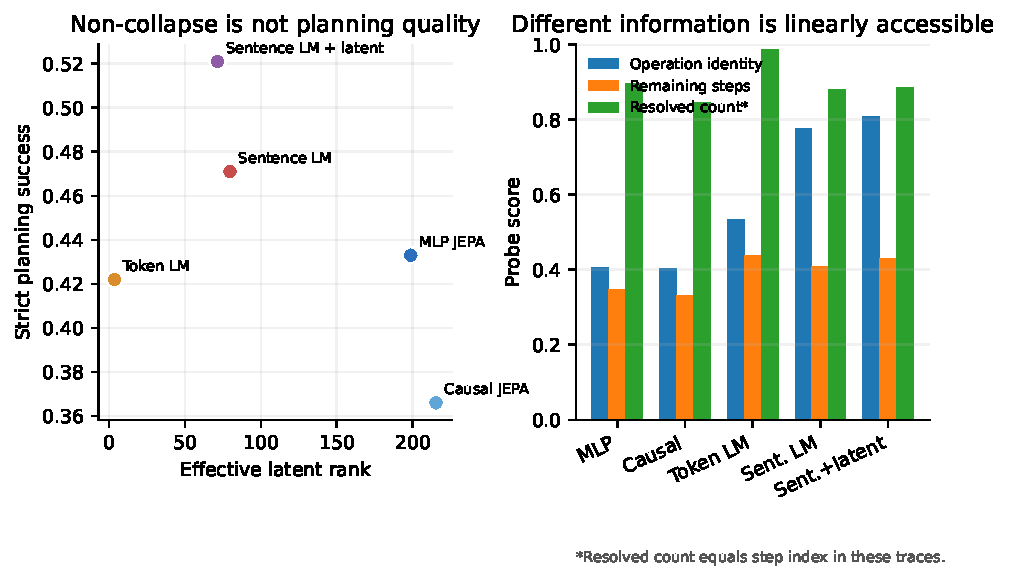
\includegraphics[width=\linewidth]{figures/representation_diagnostics.pdf}
\caption{Five-seed frozen-feature diagnostics. Effective rank is not aligned with planning success. Sentence objectives make operation identity more accessible, while all systems expose progress-related variables. Resolved count remains confounded with elapsed step index.}
\label{fig:representations}
\end{figure}

\begin{table}[h]
\caption{Paper-suite completion matrix. Empty entries are intentional.}
\label{tab:completion}
\centering
\small
\begin{tabular}{lcccc}
\toprule
Experiment family & Stylized iGSM & Faithful iGSM & ProofWriter & Blocksworld / ALFWorld \\
\midrule
Five-seed headline & complete & \todoresult & \todoresult & \todoresult \\
Five-seed GAR ablation & complete & \todoresult & \todoresult & \todoresult \\
Local ordering audit & one seed & \todoresult & \todoresult & \todoresult \\
Length OOD & partial & \todoresult & \todoresult & \todoresult \\
Controlled minimal pairs & \todoresult & \todoresult & \todoresult & \todoresult \\
Test-time FLOP scaling & repaired pilot & \todoresult & \todoresult & \todoresult \\
\bottomrule
\end{tabular}
\end{table}

\section{Predeclared analyses and decision rules}

\paragraph{Local planning geometry.}
For every feasible action pair at aligned histories, report pairwise ranking accuracy, top-1 optimal recall, mean action regret, Spearman correlation with exact continuation cost, and the optimal-versus-best-suboptimal margin. Across seeds and retained checkpoints, correlate each quantity with strict planning success. Compare those correlations with one-step latent error, successor retrieval, effective rank, and global probes. The geometry account is supported only if local ordering and margin track success materially better.

\paragraph{Gradient routing and factorization.}
Compare transition-value GAR, detached-body GAR, raw-distance GAR, and direct GAR. All learned scorers receive the same histories, candidate phrases, counterfactual outcomes, ordering labels, and tuning budget. Full geometry shaping requires a gain over detached GAR in head-free local geometry. Predictive factorization requires a gain over direct GAR on at least one preregistered axis: data efficiency, compositional length, action paraphrase, altered goals, forced-error recovery, or valid multi-step simulation.

\paragraph{Counterfactual information.}
Compare full predictive GAR, counterfactual successor prediction without GAR, shuffled GAR labels, direct GAR without successor auxiliaries, and direct GAR with the same auxiliaries. This factorial separates alternative-transition coverage, meaningful quality labels, auxiliary representation learning, and successor-mediated scoring.

\paragraph{Controlled semantic geometry.}
Construct paired histories for state paraphrase, action paraphrase, negation, operator swap, irrelevant entity renaming, and matched elapsed step with different true progress. Report full-space retrieval, normalized pairwise distances, and action-order preservation before any projection. Produce t-SNE and UMAP from the same frozen point set with shared hyperparameters across models. The projections are illustrations, not primary statistics.

\paragraph{Progress and residual structure.}
Predict remaining distance from raw goal distance, GAR energy, the full latent state, and the residual after removing the estimated progress direction. A radial-progress account requires local action ordering to degrade after removal while successor retrieval and non-progress probes remain comparatively intact.

\paragraph{Why sentence models lead.}
At aligned histories, decompose errors into candidate ranking, recovery after a forced distractor, action-type calibration, and lexical-template sensitivity. Score the sentence-plus-latent model through both its generative readout and its latent readout. This localizes whether its advantage lies in state encoding, next-phrase generation, or their combination.

\paragraph{Test-time computation.}
The scaling experiment is admitted only after a fixed-work evaluator, stable recursive transition audit, and calibrated recurrent baselines pass. Report every tested compute point on paired puzzles. A decrease with depth must first be localized to transition drift, score calibration, proposal breadth, or terminal handling. It is not presented as a test-time-scaling result by itself.

\section{Reproducibility and artifact status}

Every figure in this draft is a vector PDF. The headline, GAR, probe, and length figures are generated from the retrieved current-findings ledger. The repaired scaling figure reads the leakage-free fixed-checkpoint gate from 2026-08-04. Exact repository paths and run identifiers are recorded in the paper README. The minimal-pair panel is explicitly marked pending and contains no data.

The completed runs use immutable code snapshots and checkpoint hashes. Failed and superseded jobs remain visible in the controller ledger. The manuscript excludes the earlier candidate-length-leaking scaling curves from positive evidence. The final artifact will provide a machine-readable manifest with checkpoint path, hash, model configuration, seed, validation split, evaluation indices, parameter count, optimizer updates, wall time, and measured FLOPs for every included row.

The official ICLR 2027 style files are vendored unchanged in the paper directory. Run \texttt{make figures} through \texttt{make\_figures.sh}, then compile \texttt{main.tex} with \texttt{latexmk -pdf}. The draft remains anonymous because \texttt{\textbackslash iclrfinalcopy} is disabled.


\end{document}
